\documentclass{article}
\usepackage{graphicx}

\title{Recursion Problems}
\author{William Y. Feng}

\begin{document}

\maketitle
Of all the techniques used to solve computational contest problems, recursion is undoubtedly my favorite. In this article, we'll explore a couple of recursion problems, and I'll share some ways I like to frame them.
\begin{center}
    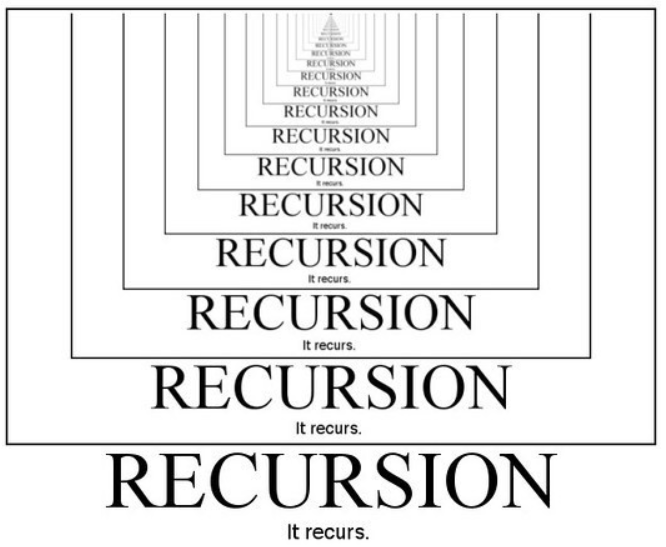
\includegraphics[scale=0.6]{images/recursion.png}
\end{center}
\textbf{Single-parameter recursion}
The simplest of recursions are those that rely on only one variable. Here's an example from the \textit{2007 AMC 12A}:

Call a set of integers spacy if it contains no more than one out of any three consecutive integers. How many subsets of $\{1,2,3,\ldots,12\},$ including the empty set, are spacy?

At a high level, the formula for recursion problems is:
\begin{enumerate}
\item Find a \textit{function} and its associated \textit{parameters} that interest us.
\item Figure out the function in terms of itself evaluated at smaller parameters—this is known as the \textbf{recurrence relation} or \textbf{state transition}.
\item Evaluate the function at increasing parameters, starting at the \textit{base cases}, and working up to what we want.
\end{enumerate}
It's not always clear where to start finding a function. Do we want \texttt{spacy\_of\_size(n)}, a function that counts the number of spacy subsets with $n$ elements? Or perhaps we want \texttt{spacy\_with\_largest(n)}, a function that counts the number of spacy subsets whose largest element is $n$.

It takes experience finding the right function to use, and often times it's not at all intuitive. For this problem, we'll use \texttt{spacy\_max(n)}, a function that counts the number of spacy subsets of $\{1, 2, 3, \dots, n\}$. (The answer to the problem is this function evaluated at $n=12$.) For the sake of concision, let's rename this function to $f(n)$; then, we have the \textit{recurrence relation}
$$f(n) = f(n - 1) + f(n - 3).$$Why is this true? Let's imagine that we're constructing a spacy subset of $\{1, 2, 3, \dots, n\}$. What choices would we make? Well, we could either include or exclude $n$.
\begin{enumerate}
\item If we include $n$, then we can't include $n - 1$ or $n - 2$ due to the spaciness condition, but we can include any lower numbers—in other words, we can tack on any subset of $\{1, 2, 3, \dots, n - 3\}$, so long as it satisfies the spaciness condition. This is precisely $f(n - 3)$.
\item If we \textit{don't} include $n$, then we can do whatever we want with the remaining numbers—in other words, we can include any subset of $\{1, 2, 3, \dots, n - 1\}$ that itself satisfies the spaciness condition. This gives $f(n - 1)$ subsets.
\end{enumerate}
And with that, we have written $f(n)$ in terms of itself, evaluated at smaller parameters. We'll often find ourselves doing this sort of casework to break down the recurrence relation.

Now all that remains is a straightforward computation of $f(12)$. I like to start by evaluating $f(1), f(2)$, etc. and work my way up, keeping my previous computations \textit{cached} in a table. For instance, here's what the table would look like for while computing $f(6)$ (clipped):
\begin{table}
    \centering
    \begin{tabular}{c|c|c|c|c|c|c|c}
         $n$ & 1 & 2 & 3 & 4 & 5 & 6 & \dots \\\hline
         $f(n)$ & 2 & 3 & 4 & 6 & 9 & & \dots
    \end{tabular}
\end{table}
Computing $f(6)$ is then as simple as looking up the values of $f(5)$ and $f(3)$, and summing them. Completing the table gives $f(12) = 129$.

\textbf{Multi-parameter recursion}
Some problems utilize recursion with \textit{multiple} parameters. Here's an example from the \textit{2016 AIME II}:

\textit{The figure below shows a ring made of six small sections which you are to paint on a wall. You have four paint colors available and you will paint each of the six sections a solid color. Find the number of ways you can choose to paint the sections if no two adjacent sections can be painted with the same color.}
\begin{center}
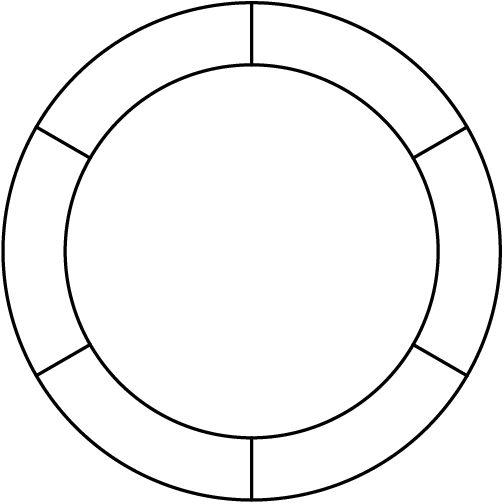
\includegraphics[scale=0.35]{images/2016_aime_ii_p12.png}
\end{center}

Let's first define the function:
\begin{enumerate}
    \item We want some function that depends on multiple parameters and counts the number of ways to paint \textit{something}.
    \item Now that we've gotten a taste of what recursion looks like, it seems natural that one parameter we should recurse on changes the \textit{size} of the problem. In this case, we'll let the parameter $n$ restrict ourselves to the first $n$ sections on the ring (starting, say, at the upper-right section).
    \item Paint colors are also a thing, so let's create another parameter, $k$, that determines what color of paint we must use in the last section painted. This is motivated because our choice of paint for a section depends on the paint used for the last section painted.
\end{enumerate}
We thus have a function, $f(n, k)$ that counts the number of ways to paint the first $n$ sections, where the last color must be color $k$. (We have numbered the paints 1, 2, 3, and 4.)

We have one minor complication, however. This is a \textit{ring}, so our choices of paint for the sixth section depend on the color of the first section. To deal with this, we exploit some symmetry—if we \textit{fix} the paint of the first section to be, without loss of generality, paint 1, then we know the last section must be painted with paints 2, 3, or 4. Thus, we impose one additional condition on $f$: now, $f(n, k)$ counts what it did before, but the first section must be color 1. Our answer will therefore be
$$4 \cdot (f(6, 2) + f(6, 3) + f(6, 4))$$
as we need to paint all 6 sections, but the last section cannot be color 1, and we multiply by 4 to account for the fact that we chose the first section to be color 1 arbitrarily.

What's our recurrence relation? Casework can help us here! To find $f(n, k)$, the number of ways to paint the first $n$ sections where the last section is color $k$ and the first section is color 1, consider that we have to have first painted the first $n - 1$ sections, and the last section cannot have been color $k$. Thus, we simply sum up the number of ways to paint $n - 1$ sections with the last section a color $i \neq k$:
$$f(n, k) = \sum_{i \neq k}^{n} f(n - 1, i).$$
We can use a table for this! Here's the table in the midst of evaluating $f(5, k)$:
\begin{center}
    %% Thanks, https://artofproblemsolving.com/wiki/index.php/2016_AIME_II_Problems/Problem_12
    \begin{tabular}{c|c|c|c|c }
        \multicolumn{1}{c}{}&\multicolumn{4}{c}{\(k\)}\\
        \(n\)&1 & 2 & 3& 4 \\ \hline
        1& 1 & 0 & 0 & 0\\
        2 & 0 & 1 & 1 & 1 \\
        3& 3 & 2 & 2 & 2 \\
        4 & 6 & 7 & 7 & 7 \\
        5 & & & & \\
        6& & & & \\
    \end{tabular}
\end{center}
To find $f(5, 1)$, for instance, we sum up the three 7s under $k=2, 3, 4$ in the previous row to get 21. To find $f(5, 2)$, we sum up $6 + 7 + 7 = 20$. Again, caching our computations in a table eliminates redundant computations.

A note about the base case for this problem: $f(1, 1) = 1$ while $f(1, 2) = f(1, 2) = f(1, 3) = 0$ because we specified that in all colorings that $f$ counts, the first segment must be color 1. Completing the table gives the answer of \textit{732}.

The exact same technique can be used on problem 16 from the 2011 AMC 12A:
\begin{quote}
    Each vertex of convex pentagon $ABCDE$ is to be assigned a color. There are $6$ colors to choose from, and the ends of each diagonal must have different colors. How many different colorings are possible?
\end{quote}
Try to use multi-parameter recursion to solve this problem!

\textbf{Conclusion}

Approaching problems with recursion has given me a more methodical and robust problem-solving strategy; it's helped reduce casework and computation while increasing confidence in my answer.

In addition to contest math, recursion is an extremely useful concept in \textit{competitive programming} as well, in the form of \textit{dynamic programming}\footnote{\url{https://en.wikipedia.org/wiki/Dynamic\_programming}}. The scale of function parameters is much larger in programming problems, but the core principle of finding a function, figuring out its recurrence relation, and computing the answer.
\end{document}